\documentclass[border=0pt]{standalone}
\usepackage{fontspec}
\setmainfont{Liberation Serif}
\usepackage{unicode-math}
\setmathfont{latinmodern-math.otf}
\usepackage{tkz-euclide}
\usetikzlibrary{arrows.meta,calc,intersections,decorations.markings,angles,quotes}

% tkz-euclide assumes centimetre coordinates. Fonts and strokes use print sizes.
\tikzset{
  every picture/.style={x=1cm,y=1cm,line width=.55pt,line cap=round,line join=round,font=\fontsize{11}{13}\selectfont},
  every node/.style={inner sep=2pt},
  construction/.style={densely dashed,line width=.4pt},
  dimension/.style={<->,>=Stealth,line width=.4pt},
  vector/.style={postaction=decorate,decoration={markings,mark=at position .55 with {\arrow{Stealth[length=4pt,width=3pt]}}}},
  note/.style={font=\fontsize{9}{11}\selectfont\itshape,draw=black!65,line width=.35pt,inner sep=3pt,align=center},
  point/.style={circle,fill=black,inner sep=0pt,minimum size=1.8pt},
  axis/.style={-{Stealth[length=4pt,width=3pt]},line width=.45pt}
}
\newcommand{\NotToScale}[1]{\node[note] at #1 {Diagram is\\NOT to scale};}
% Fix the output canvas so Typst does not resize typography to fit label extents.
\newcommand{\ExamBounds}[2]{\pgfresetboundingbox\path[use as bounding box] (0,0) rectangle (#1mm,#2mm);}

\begin{document}
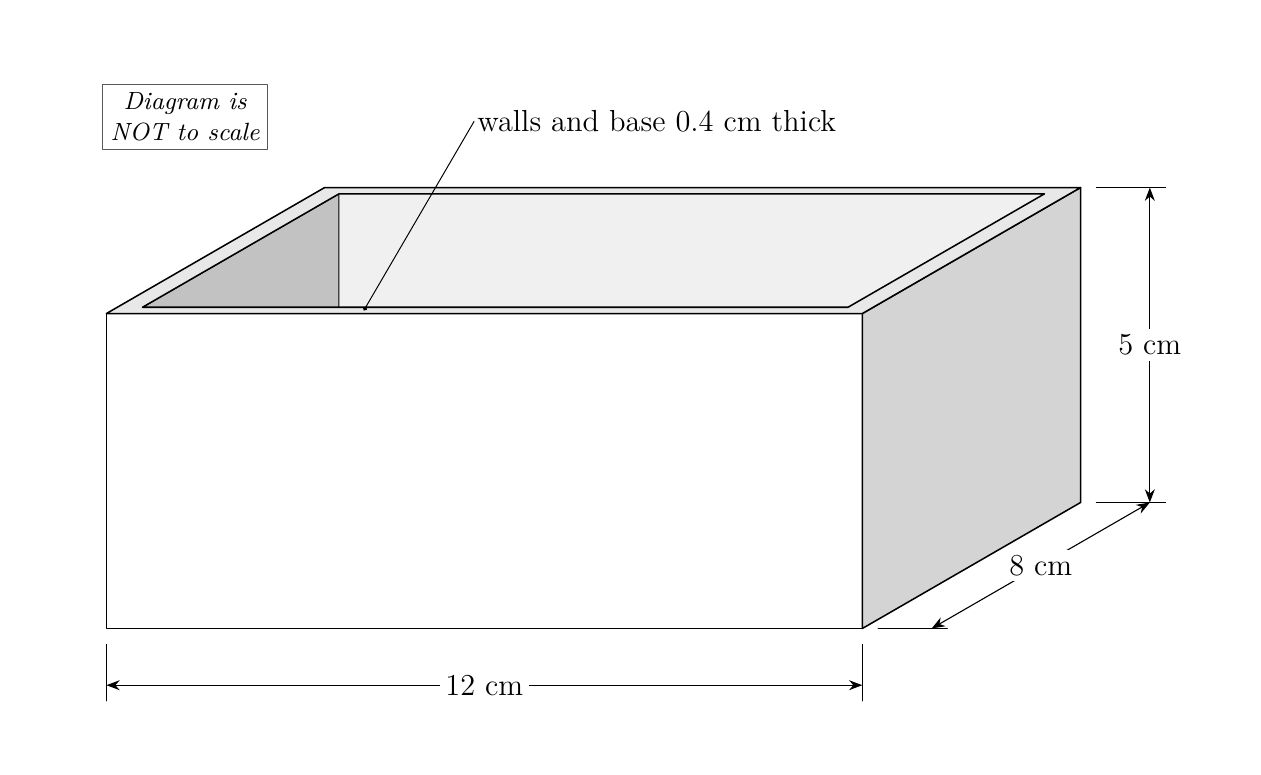
\begin{tikzpicture}
  % Page coordinates in cm. Oblique scope: 8 mm per cm, depth at 30 degrees, half scale.
  \begin{scope}[shift={(1,1.5)},x={(8mm,0mm)},y={(3.464mm,2mm)},z={(0mm,8mm)}]
    \def\t{.4}
    \coordinate (O) at (0,0,0);
    % Cavity seen through the opening: back wall, left wall and floor only.
    \begin{scope}
      \clip (\t,\t,5) -- (12-\t,\t,5) -- (12-\t,8-\t,5) -- (\t,8-\t,5) -- cycle;
      \filldraw[fill=black!13,line width=.4pt] (\t,\t,\t) -- (12-\t,\t,\t) -- (12-\t,8-\t,\t) -- (\t,8-\t,\t) -- cycle;
      \filldraw[fill=black!6,line width=.4pt] (\t,8-\t,\t) -- (12-\t,8-\t,\t) -- (12-\t,8-\t,5) -- (\t,8-\t,5) -- cycle;
      \filldraw[fill=black!24,line width=.4pt] (\t,\t,\t) -- (\t,8-\t,\t) -- (\t,8-\t,5) -- (\t,\t,5) -- cycle;
    \end{scope}
    % Exterior faces.
    \filldraw[fill=white] (0,0,0) -- (12,0,0) -- (12,0,5) -- (0,0,5) -- cycle;
    \filldraw[fill=black!17] (12,0,0) -- (12,8,0) -- (12,8,5) -- (12,0,5) -- cycle;
    % Rim: outer top outline with the opening cut out.
    \filldraw[fill=black!9,even odd rule]
      (0,0,5) -- (12,0,5) -- (12,8,5) -- (0,8,5) -- cycle
      (\t,\t,5) -- (12-\t,\t,5) -- (12-\t,8-\t,5) -- (\t,8-\t,5) -- cycle;
    % Dimensions.
    \draw[line width=.3pt] (0,0,-.25) -- (0,0,-1.15) (12,0,-.25) -- (12,0,-1.15);
    \draw[dimension] (0,0,-.9) -- node[fill=white] {12 cm} (12,0,-.9);
    \draw[line width=.3pt] (12.25,0,0) -- (13.35,0,0) (12.25,8,0) -- (13.35,8,0);
    \draw[dimension] (13.1,0,0) -- node[fill=white] {8 cm} (13.1,8,0);
    \draw[line width=.3pt] (12.25,8,5) -- (13.35,8,5) (12.25,8,0) -- (13.35,8,0);
    \draw[dimension] (13.1,8,0) -- node[fill=white] {5 cm} (13.1,8,5);
    \coordinate (rim) at (4,\t/2,5);
  \end{scope}
  \draw[line width=.35pt,{Circle[length=1.6pt]}-] (rim) -- ++(1.4,2.4) node[right,inner sep=1pt] {walls and base 0.4 cm thick};
  \NotToScale{(2,8)}
  \ExamBounds{153}{91.30645}
\end{tikzpicture}
\end{document}
